\documentclass[14pt,a4paper]{article}
\usepackage[14pt]{extsizes}
\usepackage[left=1.5cm, right=1.5cm, top=1.5cm, bottom=1.5cm]{geometry}
\usepackage[utf8]{inputenc}
\usepackage[T2A]{fontenc}
\usepackage[english, russian]{babel}
\usepackage{amsmath,amsfonts,amssymb,amsthm,mathtools} 
\usepackage{amsfonts}
\usepackage{amssymb}
\usepackage{titleps}
\usepackage{hyperref}
\usepackage{float}
\usepackage{graphicx}
\usepackage{multirow}
\usepackage{hhline}
\usepackage{wrapfig}
\usepackage{tikz}
\usepackage{pgfplots}
\usepackage{xcolor}
\usepackage{subfig}
\usepackage{upgreek}

\newcommand{\w}[1]{\text{#1}}
\newcommand{\und}[1]{\underline{#1}}
\newcommand{\img}[3]{
	\begin{figure}[H]
	\begin{center}
	\includegraphics[scale=#2]{#1}
	\end{center}
	\begin{center}
 	\textit{#3}
	\end{center}
	\end{figure}
}
\newcommand{\aw}[1]{
	\begin{center}
	\textit{#1}
	\end{center}
	\n
}
\newcommand{\be}[1]{
	\begin{center}
	\boxed{#1}
	\end{center}
}
\newcommand{\beb}[1]{
	\begin{equation}
	\boxed{#1}
	\end{equation}
}
\newcommand{\eb}[1]{
	\begin{equation}
	#1
	\end{equation}
}
\newcommand{\n}{\hfill \break}
\newcommand{\x}{\cdot}
\begin{document}

\section*{Работа 3.7.1}	
	\section*{Скин-эффект}
    \section*{Киркича Андрей, Б01-202, МФТИ}

\textbf{В работе используются}: генератор сигналов АКИП–3420, соленоид, намотанный на полый цилиндрический каркас, медный экран в виде полого цилиндра, измерительная катушка, амперметр, вольтметр, двухканальный осциллограф GOS–620, RLC-метр.

\section*{Теоретические сведения}

\ \ \ \ Толщина скин-слоя проводника:
\begin{equation}
    \delta = \sqrt{\frac{2}{\omega\sigma\mu\mu_0}}.
    \label{eq:delta}
\end{equation}

Связь полей внутри и снаружи цилиндра:
\begin{equation}
    H_1 = \frac{H_0}{\ch(\alpha h) + \frac{1}{2} \alpha a \sh(\alpha h)} 
    \text{;\ \ \ }
    \alpha = \sqrt{i\omega \sigma \mu_0} = \frac{\sqrt{2}}{\delta}e^{i\pi/4}.
    \label{eq:svyaz_poley}
\end{equation}

Отношение амплитуд полей:
\begin{equation}
    \frac{|H_1|}{|H_0|} = c \cdot \frac{U}{\nu I} = c \xi.
    \label{eq:otnoshenie_amplitud}
\end{equation}

\begin{figure}[h]
    \centering
    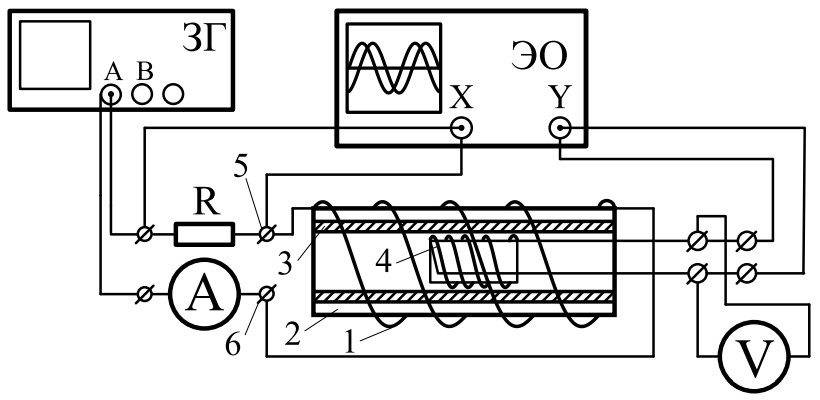
\includegraphics[width=17cm, height=8cm]{Pictures/scheme.jpg}
    \label{fig:scheme}
\end{figure}

\section*{Результаты измерений}

Перед началом работы запишем данные установки и вычислим необходимую нам для измерений частоту $\nu_h$ по формуле (1), приняв $\delta = h$.

\begin{table}[!ht]
\centering
    \begin{tabular}{|r|r|r|r|r|r|}
    \hline
        $d_{\text{нар}}, \ \text{мм}$  & $d_{\text{стен}}, \ \text{мм}$ & $\sigma, \  \frac{\text{См}}{\text{м}}$ & $\nu_{\text{h}}, \ \text{кГц} $ & $\nu_0, \ \text{Гц}$ & $\text{A}, \ \text{В}$ \\ \hline
        45 & 1,5 & 0,08 & 2,2 & 22 & 8 \\ \hline
    \end{tabular}
\end{table}
Далее приступим к измерению проводимости разными методами.
\subsection*{Измерение проводимости через отношение амплитуд}
Снимем зависимость тока через амперметр и напряжения на вольтметре от частоты, выставляемой на генераторе. Подсчитаем $\xi$, руководствуясь формулой (3).

\begin{table}[!ht]
    \centering
    \begin{tabular}{|c|r|r|r|r|r|r|r|r|r|r|}
    \hline
        $\nu, \text{Гц}$ & 22 & 30 & 40 & 50 & 60 & 70 & 80 & 90 & 100 & 110 \\ \hline
        $I, \text{А}$ & 0,53 & 0,53 & 0,52 & 0,51 & 0,51 & 0,40 & 0,49 & 0,48 & 0,47 & 0,46 \\ \hline
        $U, \text{В}$ & 0,16 & 0,22 & 0,29 & 0,36 & 0,42 & 0,47 & 0,51 & 0,55 & 0,59 & 0,62 \\ \hline
        $\xi \cdot 10^{-2}$ & 1,44 & 1,43 & 1,41 & 1,39 & 1,37 & 1,34 & 1,31 & 1,28 & 1,25 & 1,22 \\ \hline
    \end{tabular}
\end{table}

В области частот $\nu \ll \nu_h$ $\alpha h \ll 1$. Из формулы (2) получаем:

\[ (c\xi)^2 \approx \frac{1}{1+A\nu^2} \quad \Leftrightarrow \quad  \frac{1}{\xi^2}=B\nu^2 + c^2, \text{ где } B=\pi a h \sigma \mu_0 c. \]

\begin{figure}[h]
    \centering
    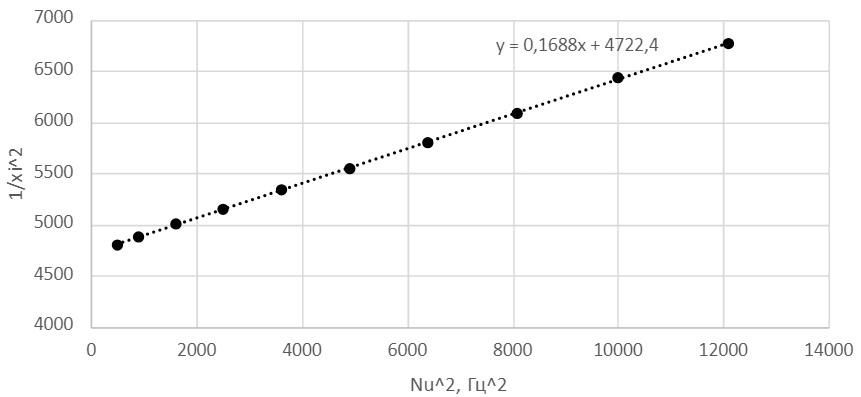
\includegraphics[width=18cm, height=8cm]{Pictures/graph1.jpg}
    \label{fig:scheme}
\end{figure}

Рассчитанное значение индуктивности: $B = (1,7\pm0,3) \x 10^{-1} \ 1/\text{Гц}^2$. Значит, $\sigma = (4,2\pm0,7) \cdot 10^7 \ \text{См/м}$ и $c = 69 \pm 10$.  

\subsection*{Измерение проводимости через разность фаз на низких частотах}
Измерим ток и напряжение в зависимости от частоты, параллельно считывая с осциллографа величину фазового сдвига $\psi$.

\begin{table}[!ht]
    \centering
    \resizebox{\textwidth}{!}{
    \begin{tabular}{|r|r|r|r|r|r|r|r|r|r|r|r|r|r|r|r|}
    \hline
        $\nu, \text{Гц}$ & 110 & 130 & 150 & 170 & 190 & 210 & 220 & 330 & 440 & 550 & 660 & 770 & 880 & 990 & 1100 \\ \hline
        $I, \text{мА}$ & 462 & 432 & 421 & 411 & 403 & 395 & 392 & 369 & 355 & 344 & 335 & 326 & 317 & 308 & 299 \\ \hline
        $U, \text{В}$ & 620 & 650 & 689 & 720 & 743 & 761 & 768 & 811 & 819 & 814 & 802 & 787 & 768 & 749 & 730 \\ \hline
        $\xi \cdot 10^{-2}$ & 1,22 & 1,16 & 1,09 & 1,03 & 0,97 & 0,92 & 0,89 & 0,67 & 0,52 & 0,43 & 0,36 & 0,31 & 0,28 & 0,25 & 0,22 \\ \hline
        $\phi, \ \text{рад}$ & 0,98 & 0,81 & 0,79 & 0,63 & 0,64 & 0,63 & 0,72 & 0,39 & 0,29 & 0,22 & 0,16 & 0,13 & 0,11 & 0,04 & 0,00 \\ \hline
        $\psi, \ \text{рад}$ & -0,59 & -0,76 & -0,79 & -0,94 & -0,93 & -0,94 & -0,85 & -1,19 & -1,28 & -1,35 & -1,41 & -1,45 & -1,47 & -1,53 & -1,57 \\ \hline
    \end{tabular}
    }
\end{table}

На основе данных из таблицы строим график на низких частотах.

\begin{figure}[h]
    \centering
    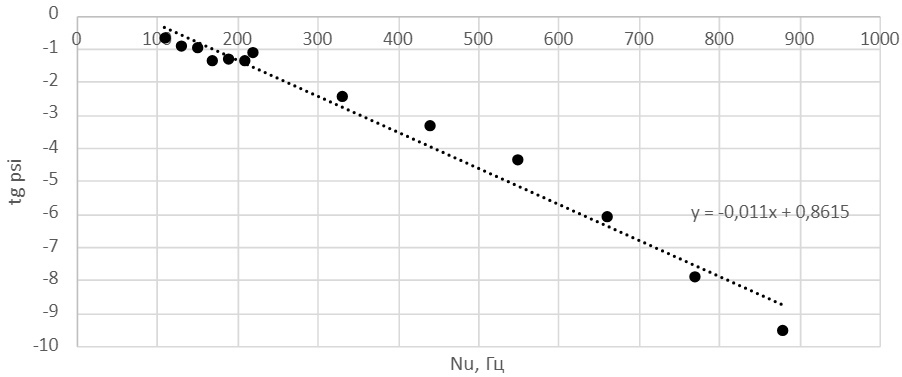
\includegraphics[width=18cm, height=9cm]{Pictures/graph2.jpg}
    \label{fig:scheme}
\end{figure}

Согласно формуле $tg \psi = \pi a h \sigma \mu_0 \nu$ получаем, что $\sigma = (8,3\pm1,3) \cdot 10^7$ См/м.

\subsection*{Измерение проводимости через разность фаз на высоких частотах}
Повторим измерения для более высоких частот.

\begin{table}[!ht]
    \centering
    \resizebox{\textwidth}{!}{
    \begin{tabular}{|r|r|r|r|r|r|r|r|r|r|r|r|r|r|r|r|}
    \hline
        $\nu, \text{Гц}$ & 1100 & 1300 & 1700 & 2200 & 2800 & 3500 & 4400 & 5500 & 7000 & 8700 & 11000 & 14000 & 17000 & 22000 & 28000 \\ \hline
        $I, \text{мА}$ & 299 & 277 & 249 & 219 & 187 & 157 & 129 & 105 & 84 & 67 & 52 & 39 & 28 & 18 & 9 \\ \hline
        $U, \text{В}$ & 730	& 676 & 609 & 532 & 452 & 374 & 303 & 239 & 184 & 140 & 104 & 76 & 57 & 48 & 46 \\ \hline
        $\xi \cdot 10^{-3}$ & 2,22 & 1,76 & 1,40 & 1,11 & 0,88 & 0,69 & 0,54 & 0,41 & 0,32 & 0,24 & 0,18 & 0,14 & 0,12 & 0,12 & 0,19 \\ \hline
        $\phi, \ \text{рад}$ & 0,00 & 0,09 & 0,14 & 0,26 & 0,39 & 0,50 & 0,86 & 1,05 & 1,41 & 1,42 & 1,48 & 1,57 & 1,69 & 1,99 & 2,35 \\ \hline
        $\psi, \ \text{рад}$ & -1,57 & -1,48 & -1,43 & -1,32 & -1,18 & -1,07 & -0,71 & -0,52 & -0,16 & -0,15 & -0,09 & 0,00 & 0,12 & 0,42 & 0,79 \\ \hline
    \end{tabular}
    }
\end{table}

\begin{figure}[H]
    \centering
    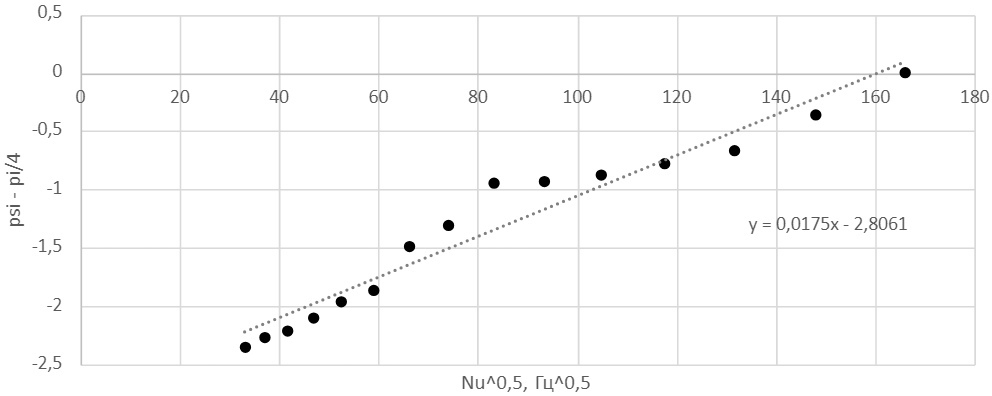
\includegraphics[width=18cm, height=9cm]{Pictures/graph3.jpg}
    \label{fig:scheme}
\end{figure}

При $\delta \ll h$ выполняется:
\begin{equation*}
    \psi - \pi/4 = k\cdot \sqrt{\nu}; \quad \ k = h\sqrt{\pi\mu_0\sigma}.
\end{equation*}
Таким образом, $k =  (1,8 \pm 0,3) \cdot 10^{-2} \ \text{рад/Гц}$, тогда $\sigma = (3,45 \pm 0,15) \cdot 10^7$ См/м.

\section*{Заключение}
В ходе выполнения работы мы проверили формулы для вычисления параметров скин-эффекта в соленоидальной катушке, вычислив отношения магнитных полей как на малых частотах токов, проходящих через катушку, так и на больших.

\section*{Литература}
\noindent
1. \textit{Сивухин Д. В.} Общий курс физики. Учеб. пособие: Для вузов. Т. III. Электричество. - 6-е издание. М.: ФИЗМАТЛИТ, 2019 \\
2. \textit{Никулин М.Г., Попов П.В., Нозик А.А., и др.} Лабораторный практикум по общей физике: учеб. пособие. В трёх томах. Т. II. Электричество и магнетизм. - 2-е издание. М.: МФТИ, 2019

\end{document}